\documentclass{beamer}
%
% Choose how your presentation looks.
%
% For more themes, color themes and font themes, see:
% http://deic.uab.es/~iblanes/beamer_gallery/index_by_theme.html
%
\mode<presentation>
{
  \usetheme{default}      % or try Darmstadt, Madrid, Warsaw, ...
  \usecolortheme{default} % or try albatross, beaver, crane, ...
  \usefonttheme{default}  % or try serif, structurebold, ...
  \setbeamertemplate{navigation symbols}{}
  \setbeamertemplate{caption}[numbered]
} 

\usepackage[english]{babel}
\usepackage[utf8x]{inputenc}
\usepackage[export]{adjustbox}% http://ctan.org/pkg/adjustbox

\graphicspath{ {img/} }

\title[Bio-inspired and Heuristic Methods]{SSCS-λ: a cellular automata-based scheduler with stochastic update based on the neighbourhood states}
\author{Tiago I. de Carvalho, \\ and Gina M. B. Oliveira}
\institute{Universidade Federal de Uberlândia}
\date{30th International Conference on Tools with Artificial Intelligence}

\begin{document}

\begin{frame}
  \titlepage
\end{frame}

% Uncomment these lines for an automatically generated outline.
% \begin{frame}{Outline}
%  \tableofcontents
% \end{frame}

\begin{frame}{Static Task Scheduling Problem (STSP)}
\begin{itemize}
  \item Assignment of tasks of a program to a multiprocessor system in order to minimize its total runtime (makespan).
  \item It has an intractable search space in the general
case.
%   \pause
  \item The system is represented by its number of processors $p$.
  \item The program is represented by a weighted directed acyclic graph $G = \{V,E,W\}$.
\end{itemize}
\end{frame}

\begin{frame}{Static Task Scheduling Problem (STSP)}
% \begin{block}{Example}
% For $p = 4$, G as the following graph.
% \end{block}

\begin{figure}
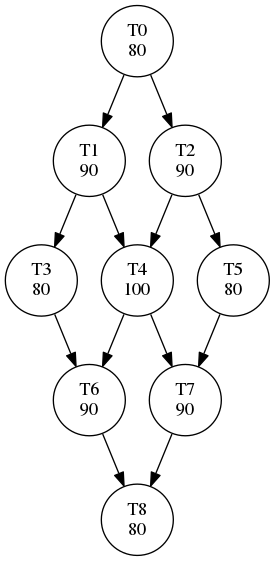
\includegraphics[width=0.28\textwidth,valign=c]{laplace9.png}%
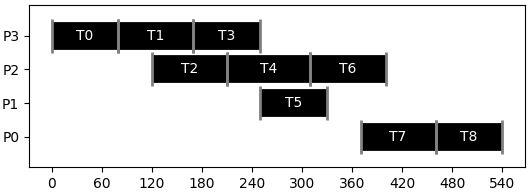
\includegraphics[width=0.80\textwidth,valign=c]{gantt_lap9.png}
\end{figure}
\end{frame}




\section{Cellular Automata}
\begin{frame}{Cellular Automata}
\begin{figure}
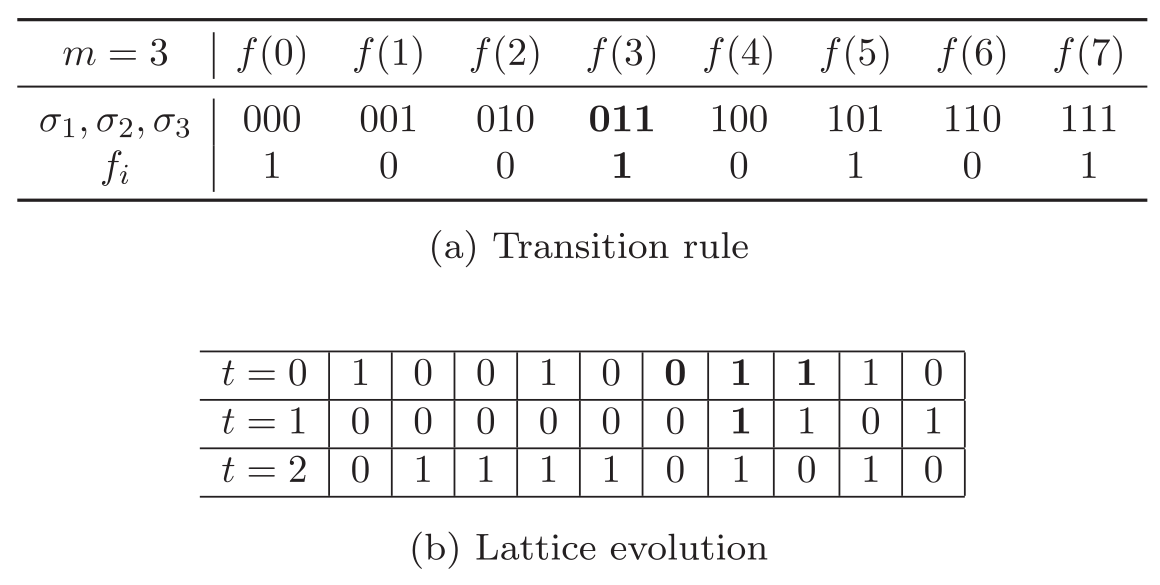
\includegraphics[width=\textwidth]{ca1.png}
\end{figure}
\end{frame}

\begin{frame}{Cellular Automata}
\begin{figure}
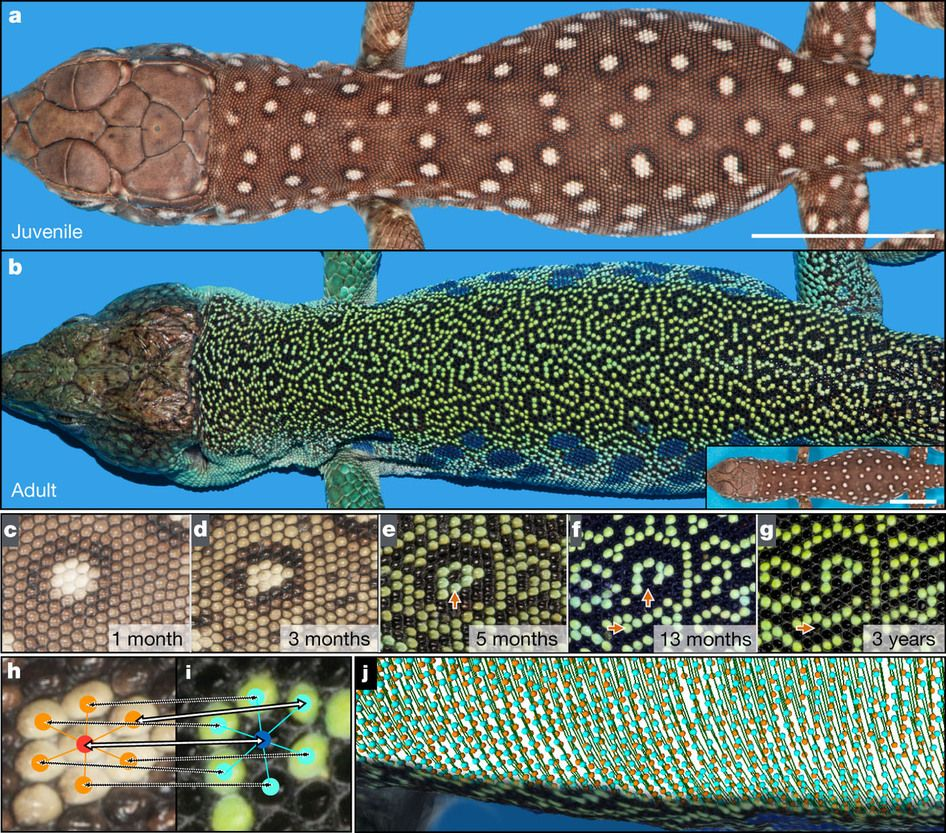
\includegraphics[width=.9\textwidth]{natural_phenomena}
\end{figure}
\end{frame}

\begin{frame}{Cellular Automata-based scheduler}
\begin{figure}
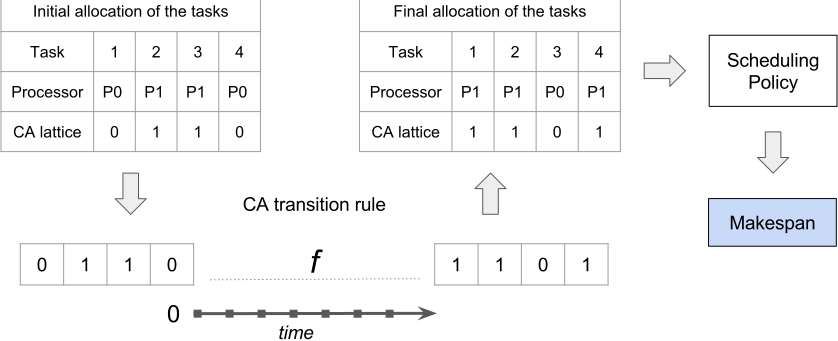
\includegraphics[width=\textwidth]{ca2.png}
\end{figure}
\end{frame}

\begin{frame}{Cellular Automata-based scheduler}
\begin{figure}
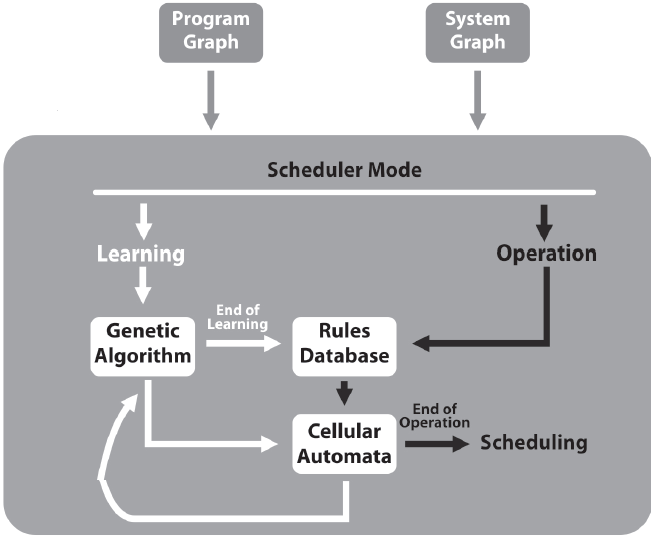
\includegraphics[width=.8\textwidth]{ca3.png}
\end{figure}
\end{frame}


\section{The reason about our investigation}
\begin{frame}{Motivation}
Current state-of-art model surpasses many methods like simple genetic algorithms and efficient heuristics. In the other hand, this scheduler has a intermediary step that rely on a random cell update that ignores the neighbours states.
\end{frame}

%\section{Benchmark set}
%\begin{frame}{Benchmark set}
%Four LAP and four FFT graphs, with \(N\) between 36 and 511, \textit{p} being 4, 8, 16 and CCR values 1.0 and 0.25. 48 instances total.
%\begin{figure}
%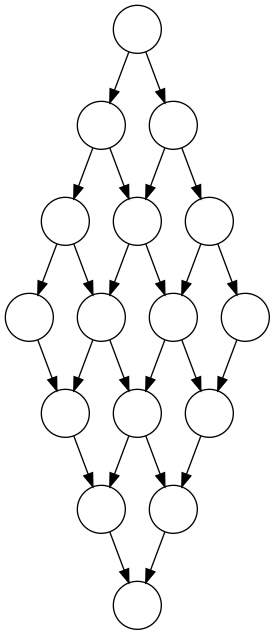
\includegraphics[width=0.28\textwidth,valign=c]{lap16.png}%
%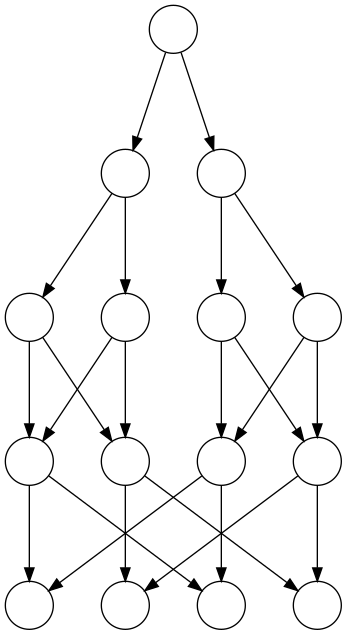
\includegraphics[width=0.35\textwidth,valign=c]{fft15.png}
%\end{figure}
%\end{frame}

\section{Genetic Algorithms}
\begin{frame}{Genetic Algorithms}
\begin{figure}
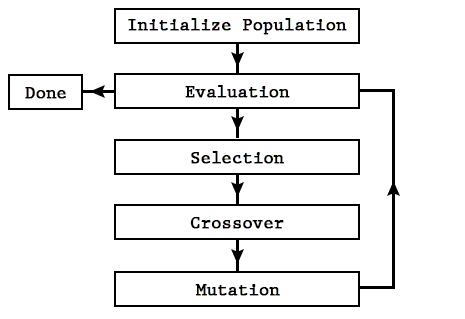
\includegraphics[width=.8\textwidth]{ga.png}
\end{figure}
\end{frame}

\begin{frame}{Standard Genetic Algorithm}
\begin{figure}
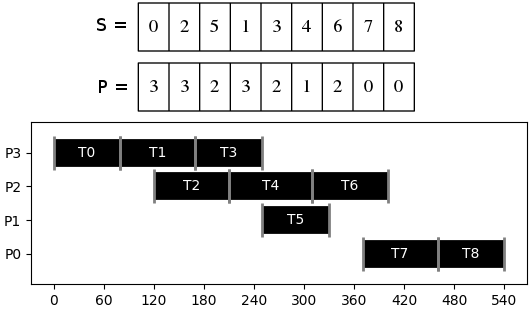
\includegraphics[width=\textwidth]{gantt_ga.png}
\end{figure}
\end{frame}

\begin{frame}{Alloc Genetic Algorithm}
\begin{itemize}
\item Evolves only the allocation of the tasks.
\item The execution order is decided by the task with the highest dynamic \textit{b-level}:
\end{itemize}
\[bl_{i} = \left\{
\begin{array}{ll}
w_{i},~\mbox{if}~i~\mbox{is~an~exit~task;} \\
\max{_{j \in successors(i)} (bl_{j} + c_{i,j}) + w_{i}},~\mbox{otherwise.}\\
\end{array}\right.
\label{eq:policy_sched}\]
\end{frame}

\section{Heuristics}
\begin{frame}{HLFET is a very efficient heuristic}
\begin{itemize}
%\item Serial heuristic: assigns every task to the same processor in an arbitrary valid execution order.
%\item Random allocation: generates 500 random task-processor assignments and uses b-level to decide execution order.
\item HLFET: a list construction heuristic that iteratively assigns the task with lowest b-level to the processor that allows its execution earliest.
\item Many studies confirm that this one of the most methods in the classical heuristic approach.
\end{itemize}
\end{frame}


\section{Methodology}
\begin{frame}{Methodology}
\begin{itemize}
\item Stochastic methods (GA, CA learning mode) were executed 100 times considering the best and average results.
\item GA parameters: $N_P = 200$, $N_G = 200$, $C_r = 65\%$, $M_r = 35\%$
\end{itemize}
\end{frame}

\section{Results}

\begin{frame}{Results}
\begin{itemize}
\item FFT graphs
	\begin{itemize}
	\item CCR = 1.0: All methods performed similarly except by the serial heuristic. \textbf{The results for R-Alloc were similar to the best methods}. 
    \item CCR = 0.25: CA was the best approach, followed by Alloc-GA.
	\end{itemize}
\item LAP graphs
	\begin{itemize}
	\item CCR = 1.0: CA was the best approach, followed by Alloc-GA and SGA.
    \item CCR = 0.25: CA was the best approach, followed by Alloc-GA and HLFET.
	\end{itemize}
\end{itemize}
\end{frame}

\section{Conclusions}
\begin{frame}{Conclusions}
\begin{itemize}
\item FFT graphs with CCR = 1.0 are not suitable for performance evaluation.
\item A significantly better performance is returned by the CA-
based scheduler for all investigated graphs.
\end{itemize}
\end{frame}

\section{Limitations and future work}
\begin{frame}{Limitations and future work}
\begin{itemize}
\item GA parameters were modest and did not scale with input size, while the CA learning process took hours.
\item Further studies will consider:
	\begin{itemize}
	\item adequate parameters for GA;
    \item more CCR values;
    \item other graphs;
    \item more sophisticated bio-inspired methods.
	\end{itemize}
\end{itemize}
\end{frame}

\begin{frame}[b]{}
\centering
\huge Thank You
\linebreak
\linebreak
\linebreak
% \linebreak
% \linebreak
% \linebreak
\begin{figure}
\centering

\includegraphics[width=.25\textwidth,valign=c]{ufu} \hspace{.1\textwidth}

\includegraphics[width=.10\textwidth,valign=c]{capes} \hspace{.1\textwidth}

\includegraphics[width=.18\textwidth,valign=c]{cnpq} \hspace{.1\textwidth}

\includegraphics[width=.10\textwidth,valign=c]{fapemig} 
\end{figure}
\end{frame}

\begin{frame}{Results}
\begin{figure}
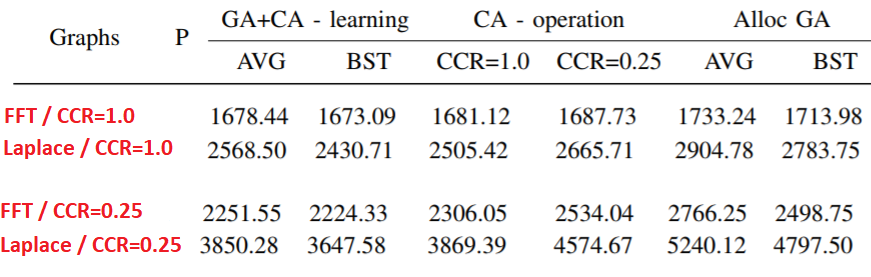
\includegraphics[width=\textwidth]{table1}
\end{figure}
\begin{figure}
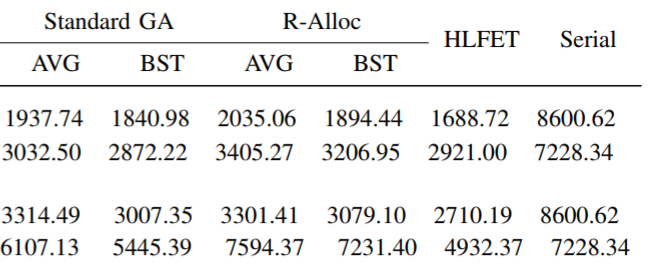
\includegraphics[width=.75\textwidth,right]{table2}
\end{figure}
\end{frame}

% \begin{frame}{Introduction}

% \begin{itemize}
%   \item Your introduction goes here!
%   \item Use \texttt{itemize} to organize your main points.
% \end{itemize}

% \vskip 1cm

% \begin{block}{Examples}
% Some examples of commonly used commands and features are included, to help you get started.
% \end{block}

% \end{frame}

% \section{Some \LaTeX{} Examples}

% \subsection{Tables and Figures}

% \begin{frame}{Tables and Figures}

% \begin{itemize}
% \item Use \texttt{tabular} for basic tables --- see Table~\ref{tab:widgets}, for example.
% \item You can upload a figure (JPEG, PNG or PDF) using the files menu. 
% \item To include it in your document, use the \texttt{includegraphics} command (see the comment below in the source code).
% \end{itemize}

% Commands to include a figure:
%\begin{figure}
%\includegraphics[width=\textwidth]{your-figure's-file-name}
%\caption{\label{fig:your-figure}Caption goes here.}
%\end{figure}

% \begin{table}
% \centering
% \begin{tabular}{l|r}
% Item & Quantity \\\hline
% Widgets & 42 \\
% Gadgets & 13
% \end{tabular}
% \caption{\label{tab:widgets}An example table.}
% \end{table}

% \end{frame}

% \subsection{Mathematics}

% \begin{frame}{Readable Mathematics}

% Let $X_1, X_2, \ldots, X_n$ be a sequence of independent and identically distributed random variables with $\text{E}[X_i] = \mu$ and $\text{Var}[X_i] = \sigma^2 < \infty$, and let
% $$S_n = \frac{X_1 + X_2 + \cdots + X_n}{n}
%       = \frac{1}{n}\sum_{i}^{n} X_i$$
% denote their mean. Then as $n$ approaches infinity, the random variables $\sqrt{n}(S_n - \mu)$ converge in distribution to a normal $\mathcal{N}(0, \sigma^2)$.

% \end{frame}

\end{document}
